% !TEX encoding = UTF-8
% !TEX TS-program = pdflatex
% !TEX root = ../tesi.tex

%**************************************************************
\chapter{Contesto aziendale}
\label{cap:contesto-aziendale}
%**************************************************************

% \noindent Esempio di utilizzo di un termine nel glossario \\
% \gls{api}. \\
%
% \noindent Esempio di citazione in linea \\
% \cite{site:agile-manifesto}. \\
%
% \noindent Esempio di citazione nel pie' di pagina \\
% citazione\footcite{womak:lean-thinking} \\

%**************************************************************
\section{Introduzione}

In questo documento descrivo la mia esperienza di \textit{stage} presso la sede di Padova di \textbf{Sync Lab}, un'azienda nata come \textit{software house} e che, negli anni, si è affermata nel campo dell'\textit{ICT} (\textit{Information and Comunication Technology}).\\
È di particolare rilievo, nella mia particolare esperienza, il periodo storico in cui questo tirocinio è avvenuto: ho infatti effettuato lo stage tra il mese di settembre e il mese di ottobre 2020, ossia durante l'emergenza sanitaria globale dovuta alla malattia \textit{COVID-19}. La pandemia in atto ha influenzato radicalmente il lavoro di molte persone, me compreso: al fine di ridurre le possibilità di contagio, infatti, ho dovuto svolgere gran parte del tirocinio in regime di \textit{smart working}, potendo accedere alla struttura solo una volta alla settimana, e alle infrastrutture quasi esclusivamente in maniera remota.
Nonostante la situazione non favorevole, ho avuto comunque modo di interfacciarmi con i dipendenti dell'azienda; sono quindi riuscito anche a raccogliere le informazioni riguardanti l'azienda che, unite a delle ricerche online, ho riportato in questo capitolo.

\section{L'azienda}

Sync Lab nasce come \textit{software house} a Napoli nel 2002; negli anni, l'azienda si espande a gran velocità, aprendo sedi a Roma, Milano, Padova e Verona. Al giorno d'oggi, l'azienda conta 5 sedi, per un totale di oltre 250 dipendenti e più di 150 clienti diretti e finali. \\
Dall'apertura ad oggi, Sync Lab si è tramutata in un \textit{system integrator} grazie alla maturazione delle competenze tecniche e metodologiche in ambito software. Un tratto distintivo dell'azienda è la grande attenzione posta alla gestione delle \textbf{risorse umane}: testimonianza di ciò è il basso \textit{turn-over}, segno che i collaboratori condividono un progetto comune e concreto. \\
Altro segno d'eccellenza sono le certificazioni di qualità che l'azienda ha conseguito; finora, infatti, l'azienda ha ottenuto le certificazioni per gli standard \textit{ISO 9001}, \textit{ISO 14001}, \textit{ISO 27001} e \textit{ISO 45001}.

\subsection*{Prodotti e servizi offerti}

Una certa attenzione è posta dall'azienda alla diversificazione dei prodotti e dei servizi offerti; essi sono infatti inquadrabili in diverse aree tematiche, quali salute, \textit{privacy}, sicurezza, telecomunicazioni, finanza, territorio e ambiente. \\
Alcuni dei prodotti che l'azienda offre al momento sono i seguenti:

\begin{itemize}
  \item \textbf{DPS 4.0}: software per la gestione degli adempimenti alla \textit{Privacy GDPR - General Data Protection Regulation}, utilizzato da svariate aziende per attuare correttamente quanto previsto da tale regolamento europeo; tale prodotto permette di censire, tracciare e controllare chi può trattare dati personali in azienda;

  \item \textbf{StreamLog}: sistema finalizzato al soddisfacimento dei requisiti fissati dal \textit{Garante per la Protezione dei dati personali}, utilizzato dagli amministratori di sistema per controllare gli accessi agli utenti al fine di soddisfare i requisiti di \textit{privacy} richiesti dal garante;

  \item \textbf{SynClinic}: sistema informativo per la gestione integrata dei processi, clinici e amministrativi, di ospedali, cliniche e case di cura. Questo applicativo fornisce svariate funzionalità organizzate in moduli, elencati nell'immagine seguente, che intersecano i bisogni del personale amministrativo e quelli del personale clinico delle strutture sanitarie, permettendo di gestire e monitorare tutte le fasi del percorso di cura del paziente. È utilizzabile sia in \textit{cloud} che \textit{on premises};

  \begin{minipage}{\linewidth}
    \centering
      
\includegraphics[height=6cm]{immagini/synclinic}
    \captionof{figure}{Moduli di SynClinic.}
    \caption*{\textbf{Fonte:} synclinic.it}
  \end{minipage}

  \item \textbf{StreamCrusher}: tecnologia che aiuta le aziende a effettuare corrette decisioni di \textit{business}, a identificare tempestivamente eventuali criticità e a riorganizzare i processi in base a nuove esigenze. Questo software è in grado di raccogliere, indicizzare e interpretare i dati, siano essi \textit{log} di applicazione o di sistema, \textit{alert}, dati di configurazione o modifiche ai sistemi, al fine di estrapolarne informazioni utili all'\textit{IT management};

  \item \textbf{Wave}: software che si propone come integrazione tra il mondo della videosorveglianza e quello dei \textit{Sistemi Informativi Territoriali}, permettendo di avere una visione geo-referenziata della distribuzione delle telecamere installate sul territorio e consentendo così all'utilizzatore di avere un impatto visivo immediato sull'area di copertura di una data installazione reale, o di avere un'anteprima di tale area in fase di progettazione;

  \item \textbf{Seastream}: piattaforma pensata per migliorare l'efficienza, la sicurezza e il processo di innovazione del settore marittimo; per fare ciò l'azienda fornisce, attraverso questa piattaforma, un \textit{Fleet Operation Center (FOC)}, ovvero un sistema di monitoraggio avanzato delle flotte armatoriali operative in tutto il mondo, e un \textit{Harbor Operation Platform (HOC)}, ovvero una piattaforma di servizi per gli operatori portuali. \\

  % \begin{minipage}{\linewidth}
  %   \centering
  %     
\includegraphics[height=3.5cm]{immagini/seastream}
  %   \captionof{figure}{Funzionalità del progetto Seastream.}
  %   \caption*{\textbf{Fonte:} synclab.it}
  % \end{minipage}

\end{itemize}

\subsection*{Clienti principali}
Sync Lab collabora con numerose aziende italiane e multinazionali, sia pubbliche che private. Tra le aziende \textbf{private} più importanti possiamo trovare \textit{Sky}, \textit{Eni}, \textit{Enel}, \textit{Vodafone}, \textit{Accenture}, \textit{Fastweb}, \textit{Tim}, \textit{UniCredit} e \textit{H\&M}. \\
Tra le collaborazioni con \textbf{enti statali} e parastatali, invece, troviamo quelle con \textit{Trenitalia}, \textit{RAI}, \textit{Poste Italiane}, la \textit{Regione Lazio} e il \textit{Ministero dell'Economia e delle Finanze}.

%**************************************************************
\section{Processi aziendali}

\subsection{Processi}

L'azienda persegue i propri obiettivi attuando i processi qui elencati.

\subsubsection*{Consulenza}

L'azienda fornisce servizi di consulenza informatica a svariate imprese, sia pubbliche che private; questi servizi hanno lo scopo di far evolvere, sia in termini di sviluppo che di competitività, i clienti dell azienda. Per fare ciò, Sync Lab collabora con altre aziende di consulenza e con specialisti del settore.

\subsubsection*{Fornitura}

Il processo di fornitura viene istanziato ogniqualvolta un cliente assume Sync Lab per lo sviluppo e la realizzazione di un prodotto. Contemporaneamente alla realizzazione, l'azienda svolge delle attività che possano migliorare questo processo. In particolare:
\begin{itemize}
  \item \textbf{Qualità del software}: il software viene controllato e ottimizzato, anche attraverso l'utilizzo delle \textit{best practice}, al fine di aderire alle regole aziendali;
  \item \textbf{Verifica delle procedure}: le procedure vengono verificate, al fine di poter agire in maniera correttiva nel caso in cui si dovessero manifestare dei problemi;
  \item \textbf{Analisi e miglioramento degli standard}: gli standard aziendali vengono analizzati e, possibilmente, migliorati; conseguenza di ciò è un costante miglioramento anche dal punto di vista di qualità del software.
\end{itemize}

\subsubsection*{Sviluppo}

Per quanto riguarda il processo di sviluppo, Sync Lab fa uso della metodologia \textit{Agile}\footcite{tec:agile}, descritta più dettagliatamente in seguito. Questa permette di coinvolgere il cliente durante tutto il processo, tenendolo aggiornato sull'evoluzione dello sviluppo del prodotto e ricevendo di ritorno le sue opinioni, al fine di poter agire sia correttivamente che migliorativamente.

\subsubsection*{Manutenzione}

Una volta consegnato il prodotto, l'azienda assicura le attività di manutenzione per tutto il ciclo di vita del software. La manutenzione offerta dall'azienda è di tre tipi:
\begin{itemize}
  \item \textbf{Correttiva}, corrispondente alla correzione di eventuali difetti;
  \item \textbf{Adattiva}, ossia il riadattamento del software a nuovi requisiti quali l'ambiente di produzione o l'architettura;
  \item \textbf{Evolutiva}, ossia l'aggiunta o l'aggiornamento in senso migliorativo di porzioni di software.
\end{itemize}

\subsection{Metodologia Agile}

Per il processo di sviluppo, l'azienda fa uso di una metodologia \textit{Agile} che molto si avvicina al modello \textit{Scrum}\footcite{tec:scrum}. Punto cardine del metodo di sviluppo di Sync Lab, infatti, è la continua interazione con gli \textit{stakeholder}, ossia i clienti: questi vengono coinvolti durante tutto il processo, venendo aggiornati sull'evoluzione del prodotto; questo permette all'azienda di ricevere \textit{feedback} che possono aiutare a migliorare il prodotto e ad adattarlo al meglio alle esigenze. \\
Come ho potuto constatare di persona durante il mio periodo di tirocinio, il modello adottato dall'azienda prevede uno sviluppo che procede per \textit{sprint}, ossia un'unità di base di durata fissa compresa tra una e quattro settimane a seconda degli obiettivi posti. A ogni \textit{sprint} corrisponde una funzionalità; questa viene verificata insieme al cliente, per tastarne la soddisfazione o ricevere consigli che possano migliorare tale nuova funzionalità. \\

\begin{minipage}{\linewidth}
  \centering
    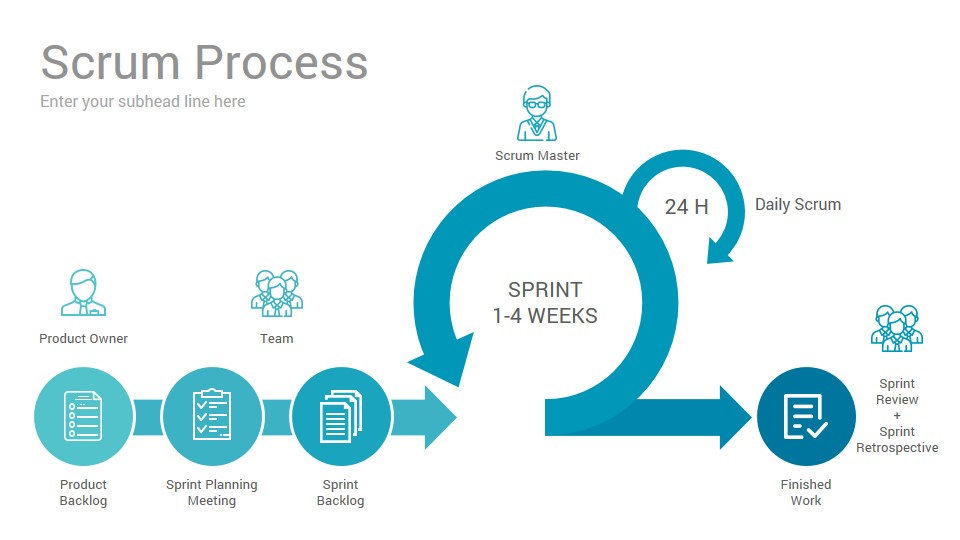
\includegraphics[height=4cm]{immagini/scrum}
  \captionof{figure}{Metodologia Scrum.}
  \caption*{\textbf{Fonte:} antevenio.com}
\end{minipage} \\

Lo sviluppo di un prodotto in Sync Lab passa attraverso cinque attività, inquadrabili tutte in quanto previsto dalla metodologia \textit{Scrum} riassunta dalla precedente immagine. \\
La prima attività che viene svolta è la redazione di una lista di cose da fare per portare a termine il progetto; nel caso del mio progetto di \textit{stage}, ad esempio, ho definito insieme al tutor aziendale le \textit{feature} che avrei dovuto mettere a disposizione, e abbiamo visionato assieme i \textit{bug} presenti nel codice che avrei dovuto utilizzare come \textit{baseline}, al fine di sapere cosa avrei dovuto correggere di quanto già fatto. Nella metodologia \textit{Scrum}, questa lista assume il nome di \textbf{Product Backlog}. \\
Dopo aver redatto questa lista, solitamente viene realizzata una pianificazione degli \textit{sprint} che è necessario effettuare per portare a termine il progetto. In ambito \textit{Scrum} questa pianificazione viene chiamata \textbf{Sprint Planning}, e nel caso del mio tirocinio è corrisposta alla divisione in incrementi che avrei dovuto effettuare per completare il piano di lavoro. Successivamente a questo, vengono individuati dei sottoinsiemi di obiettivi per ogni \textit{sprint} definito durante l'attività chiamata \textbf{Sprint Backlog}. Un esempio pratico di questa attività è la definizione degli incrementi che ho effettuato prima di cominciare lo \textit{stage}. \\
Una volta definiti tutti gli obiettivi e aver correttamente diviso le tempistiche in \textbf{Sprint}, questi vengono ad uno ad uno eseguiti; nell'ambito del mio stage, questo è corrisposto allo sviluppo di quanto previsto dal piano di progetto. All'esecuzione di ogni incremento, inoltre, di questo è stata verificata l'aderenza agli obiettivi posti, che nella metodologia \textit{Scrum} vegnono chiamati \textbf{Sprint Goal}.

Durante il mio \textit{stage} ho inoltre potuto sperimentare anche due degli eventi facenti parte della metodologia \textit{Scrum}, ossia il \textit{Daily Scrum} e lo \textit{Sprint Review}:
\begin{itemize}
  \item Il \textbf{Daily Scrum}, come definito dai creatori di questa metodologia, è un evento a cadenza giornaliera in cui i membri del gruppo di lavoro discutono dell'andamento dello \textit{sprint}. Questo evento viene svolto dai diversi \textit{team} di lavoro dell'azienda giornalmente; nel caso specifico del mio tirocinio, essendosi questo svolto in gran parte in \textit{remote working}, questo evento non ha potuto avere cadenza giornaliera. Nonstante questo, ho effettuato svariati allineamenti con il tutor aziendale, e questo si può almeno in parte configurare con quanto previsto dalla metodologia;
  \item Lo \textbf{Sprint Review}, ossia la verifica di quanto effettuato durante uno \textit{sprint} alla fine di questo, viene effettuato da tutti i gruppi di lavoro al raggiungimento degli obiettivi fissati dallo \textit{sprint}. Nel caso specifico del mio tirocinio, questo evento ha avuto luogo quasi settimanalmente, con la verifica di quanto fatto durante l'incremento definito.
\end{itemize}

%**************************************************************

\section{Tecnologie utilizzate}

Come riportato sul sito aziendale, Sync Lab fa uso di diversi linguaggi di programmazione, \textit{framework} e strumenti di supporto moderni e funzionali, al fine di soddisfare i clienti; oltre a questo, l'azienda è costantemente aggiornata sulle tecnologie di riferimento e pronta ad espandere le proprie conoscenze con le tecnologie più moderne. \newpage

\begin{minipage}{\linewidth}
  \centering
    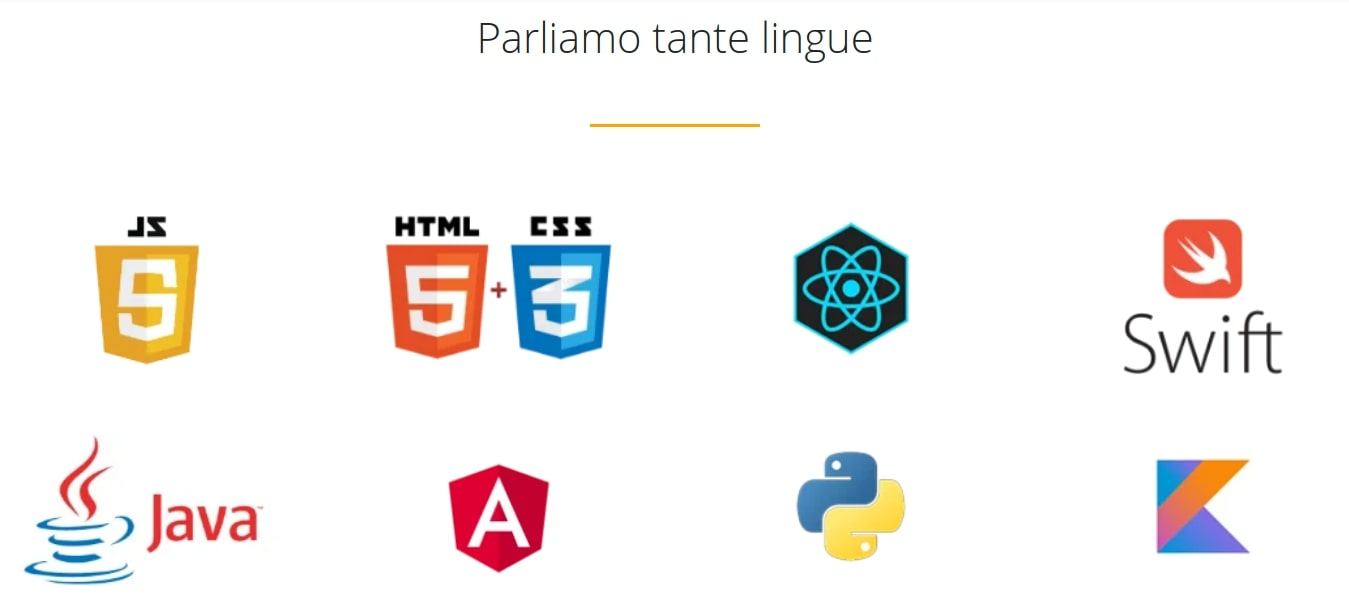
\includegraphics[height=4cm]{immagini/linguaggi}
  \captionof{figure}{Panoramica delle tecnologie utilizzate da Sync Lab.}
  \caption*{\textbf{Fonte:} synclab.it}
\end{minipage} \\

Tra i linguaggi di programmazione più utilizzati troviamo i seguenti:
\begin{itemize}
  \item \textbf{Java}\footcite{tec:java}: linguaggio di programmazione ad alto livello orientato agli oggetti, largamente utilizzato dalle aziende; in particolare, \textit{Java} viene utilizzato da Sync Lab, in accoppiata al \textit{framework Spring}\footcite{tec:spring}, per lo sviluppo dei servizi \textit{REST} necessari alle componenti \textit{back-end} di svariati applicativi, tra cui ad esempio \textit{SynClinic} e \textit{StreamCrusher}. Questo linguaggio, abbinato al \textit{framework Spring}, è stato utilizzato anche per lo sviluppo della componente \textit{back-end} dell'applicativo \textit{SyncTrace}, oggetto del mio tirocinio;

  \item \textbf{JavaScript}\footcite{tec:javascript}: linguaggio di programmazione orientato agli oggetti e agli eventi, originariamente pensato per la creazione di effetti dinamici interattivi per i siti web ma sempre più utilizzato come linguaggio \textit{general purpose} per lo sviluppo di applicativi web e non web. Viene utilizzato dall'azienda per realizzare la componente logica delle \textit{single page application};

  \item \textbf{TypeScript}\footcite{tec:typescript}: \textit{super-set} di \textit{JavaScript} sviluppato da \textit{Microsoft}. Questo linguaggio estende la sintassi di \textit{JavaScript} in modo che ogni programma scritto in \textit{JavaScript} possa funzionare anche con \textit{TypeScript}, e come il primo viene utilizzato dall'azienda per realizzare la componente logica delle \textit{single page application}. Si può trovare questo linguaggio, abbinato al \textit{framework Angular}\footcite{tec:angular}, in svariati prodotti dell'azienda, tra cui \textit{SynClinic} e \textit{DPS4.0}; è inoltre il linguaggio con il quale è stata scritta la componente \textit{front-end} della \textit{web application} di \textit{SyncTrace};

  \item \textbf{HTML5 e CSS3}\footcite{tec:htmlcss}: linguaggi di \textit{markup} utilizzati, anche dall'azienda, per modellare la componente visiva delle \textit{single page application} e, più in generale, dei siti web. Questi linguaggi di \textit{markup} sono usati dall'azienda principalmente nei progetti che coinvolgono il \textit{framework Angular}, come ad esempio \textit{SynClinic} e \textit{DPS4.0};

  \item \textbf{Kotlin}\footcite{tec:kotlin}: linguaggio di programmazione \textit{general purpose} e multi-paradigma, sviluppato da \textit{JetBrains}, utilizzato dall'azienda per sviluppare le applicazioni mobili per i dispositivi \textit{Android}. Un esempio di utilizzo di questo linguaggio è l'applicazione mobile per il \textit{contact tracing} del progetto \textit{SyncTrace};

  \item \textbf{Swift}\footcite{tec:swift}: linguaggio di programmazione orientato agli oggetti, sviluppato da \textit{Apple} e utilizzato dall'azienda per sviluppare le applicazioni mobili per i dispositivi \textit{iOS}.
\end{itemize}

L'azienda utilizza anche svariati \textit{framework} a supporto della programmazione; alcuni tra i \textit{framework} più utilizzati dall'azienda sono:
\begin{itemize}
  \item \textbf{Spring}: \textit{framework open-source} per lo sviluppo di applicazioni con linguaggio di programmazione \textit{Java}; viene utilizzato, possibilmente combinando il \textit{core} del \textit{framework} con altri progetti quali \textit{Spring Boot} e \textit{Spring Data}, per sviluppare applicativi lato \textit{server}. Esempio di utilizzo di questo \textit{framework} da parte di Sync Lab sono svariate applicazioni web la cui componente \textit{back-end} è sviluppata con l'ausilio di queste tecnologie, come ad esempio \textit{SynClinic} e \textit{StreamCrusher}. Di seguito viene riportata l'architettura generale di tale \textit{framework};

  \begin{minipage}{\linewidth}
    \centering
      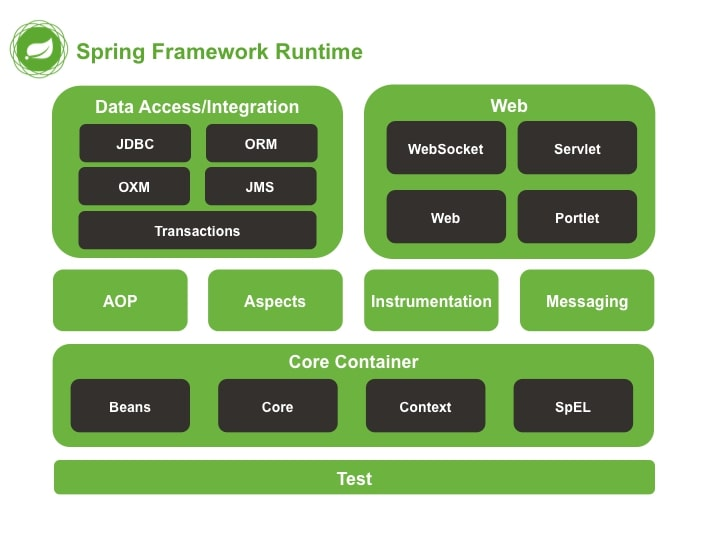
\includegraphics[height=5cm]{immagini/spring}
    \captionof{figure}{Architettura dello \textit{Spring framework}.}
    \caption*{\textbf{Fonte:} javaboss.it}
  \end{minipage}

  \item \textbf{Angular}: \textit{framework open-source} per lo sviluppo di applicazioni web tramite linguaggio di programmazione \textit{TypeScript}. L'utilizzo principale di questa tecnologia risiede nello sviluppo di \textit{single page application} reattive e costruite su un \textit{back-end} composto da servizi \textit{REST}. Esempi di utilizzo di questo \textit{framework} sono \textit{SynClinic} e \textit{DPS4.0}, già citati in precedenza. \\
  Oltre alla possibilità di sviluppare applicativi veloci e funzionali, questo \textit{framework} offre anche un \textit{design pattern} di tipo \textit{Model-View-ViewModel} nativo come riassunto dalla seguente immagine, fattore che facilita la progettazione e lo sviluppo delle applicazioni;

  \begin{minipage}{\linewidth}
    \centering
      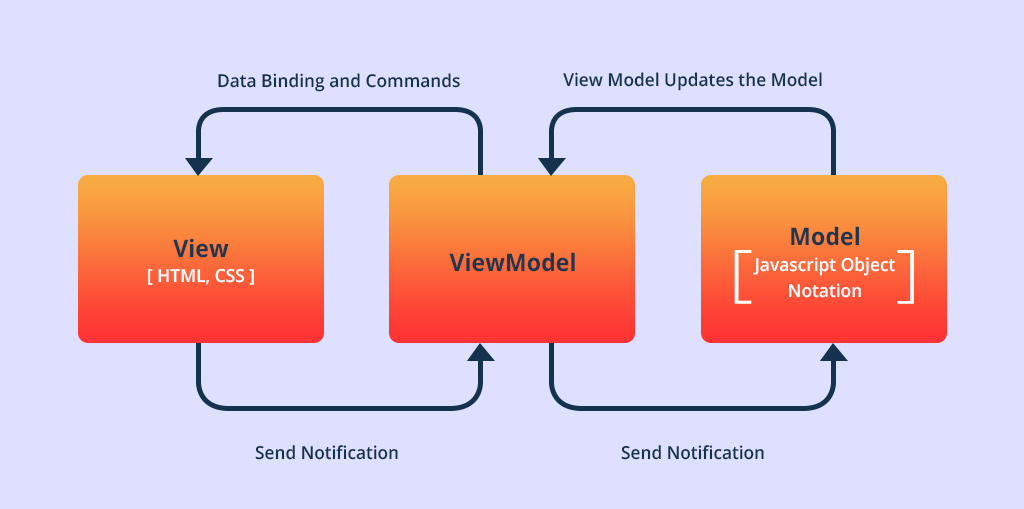
\includegraphics[height=5cm]{immagini/angular}
    \captionof{figure}{Pattern MVVM, adottato anche dal \textit{framework Angular}.}
    \caption*{\textbf{Fonte:} alphalogicinc.com}
  \end{minipage}

  \item \textbf{Electron}\footcite{tec:electron}: \textit{framework open-source} che consente lo sviluppo dell'interfaccia grafica di applicazioni desktop utilizzando tecnologie tipicamente pensate per il web, quali \textit{HTML}, \textit{CSS}, \textit{JavaScript} e \textit{TypeScript}; per fare ciò, questa tecnologia combina il motore di rendering \textit{Chromium} e il \textit{runtime} \textit{NodeJS}\footcite{tec:nodejs}. \\

  \begin{minipage}{\linewidth}
    \centering
      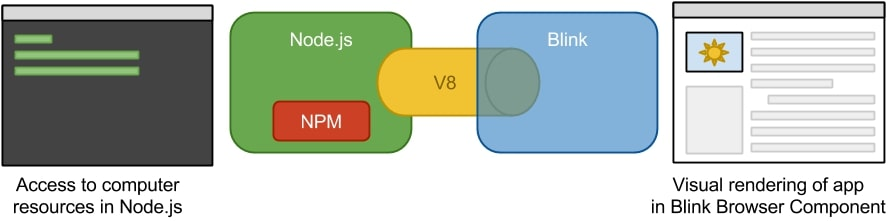
\includegraphics[height=2cm]{immagini/electron}
    \captionof{figure}{Funzionamento del \textit{framework Electron} con \textit{NodeJS}.}
    \caption*{\textbf{Fonte:} freecontent.manning.com}
  \end{minipage}
\end{itemize}

Sync Lab utilizza strumenti tecnologici anche per gestire il lavoro da remoto; in particolare, durante l'emergenza sanitaria ancora in corso, l'azienda fa uso di diverse tecnologie per organizzare il lavoro non in presenza, permettendo a tutti i collaboratori di rimanere correttamente aggiornati sulle attività e i compiti di cui sono responsabili. Alcune di queste tecnologie sono le seguenti:

\begin{itemize}
  \item \textbf{Google Meet}: servizio di \textit{Google} per effettuare videoconferenze online. Questa piattaforma viene usata dall'azienda, e in particolare è stata utilizzata anche durante il mio \textit{stage}, per comunicare con gli altri collaboratori e poter rimanere aggiornati sui progressi effettuati;

  \item \textbf{Discord}: applicazione \textit{VoIP} per la comunicazione vocale e testuale. Uno dei punti di forza di questa piattaforma, sfruttato anche dall'azienda, è la possibilità di poter avere più canali, sia testuali che vocali, all'interno dello stesso \textit{server}; questo permette una comunicazione più ordinata e metodica, riducendo il rischio di incomprensioni;

  \item \textbf{Google Docs}: servizio di \textit{Google} per la condivisione di documenti online. Questa piattaforma è stata utilizzata in particolare durante il mio tirocinio per tenere traccia degli incrementi giornalieri che ho svolto;

  \item \textbf{Trello}: software gestionale in stile \textit{Kanban}, utilizzato per coordinare il proprio \textit{workflow} e visualizzare quello degli altri collaboratori. Questa piattaforma si sposa bene con la metodologia \textit{Agile} che Sync Lab utilizza, in quanto può essere utilizzato come una \textit{Scrum board}.
\end{itemize}

%**************************************************************

\section{Propensione all'innovazione}

Sync Lab presta grande attenzione anche all'innovazione e allo sviluppo, sia in senso tecnologico che industriale. L'azienda, infatti, conta tre dipartimenti ideati per sperimentare e innovare, i quali sono \textbf{Research and Development}, nato con lo scopo di promuovere nuovi prodotti nati da ricerche in svariati settori, \textbf{Lab}, in cui l'azienda sviluppa soluzioni a quanto studiato nel precedente dipartimento, e \textbf{Start-up}, il cui scopo è quello di promuovere le \textit{start-up} di maggiore rilevanza per quanto riguarda l'innovazione; per fare ciò, Sync Lab collabora con svariati enti privati e università, sia italiane che estere. \\

\begin{minipage}{\linewidth}
  \centering
    
\includegraphics[height=2cm]{immagini/universita}
  \captionof{figure}{Alcune università con le quali l'azienda collabora.}
  \caption*{\textbf{Fonte:} synclab.it}
\end{minipage} \\

Alcuni dei progetti di ricerca fondati e mantenuti da Sync Lab sono i seguenti:
\begin{itemize}
  \item \textbf{BIG-ASC}: acronimo di \textit{BIG Data and Advanced Analytics for Secure Mobile Commerce}, è un progetto che punta a creare una piattaforma \textit{Big Data} che sappia rispondere a requisiti stringenti delle piattaforme di \textit{Mobile Commerce}, come la scalabilità, l'autonomia e le \textit{performance}, attraverso l'analisi continua e in tempo reale dei dati d'utilizzo. Per fare questo, Sync Lab collabora con l'azienda \textit{CeRICT} e l'\textit{Università degli studi Parthenope} di Napoli;
  \item \textbf{eHealthNet}: ecosistema software per la Sanità Elettronica, che si propone di intervenire su quattro aree tematiche riguardanti la sanità, ossia interoperabilità, pervasività, sostenibilità e preventivabilità. Per lo sviluppo di questo progetto è stato avviato un laboratorio che vede come collaboratori svariate aziende private, l'\textit{Istituto Italiano di Tecnologia}, l'\textit{Istituto Nazionale Tumori}, l'\textit{Università degli studi Federico II} di Napoli e l'\textit{Università degli studi di Salerno};
  \item \textbf{BDA4PHR}: piattaforma \textit{open-source}, scalabile, estendibile e manutenibile che offre servizi di \textit{storing} e \textit{Big Data Analytics} dedicati ad informazioni di tipo medico-sanitario. Lo scopo di questo progetto è la creazione di un \textit{repository} sicuro, distribuito e affidabile per la gestione, la condivisone e l'analisi di dati eterogenei. Tra i finanziatori di questo progetto ci sono l'\textit{Unione Europea} e il \textit{Ministero dello Sviluppo Economico} italiano. \\
\end{itemize}

I progetti a cui l'azienda prende parte sono molteplici e in continuo aumento; alcuni dei progetti ora attivi sono riassunti dal sito aziendale, del quale l'immagine che segue è una cattura di schermo.

\begin{minipage}{\linewidth}
  \centering
    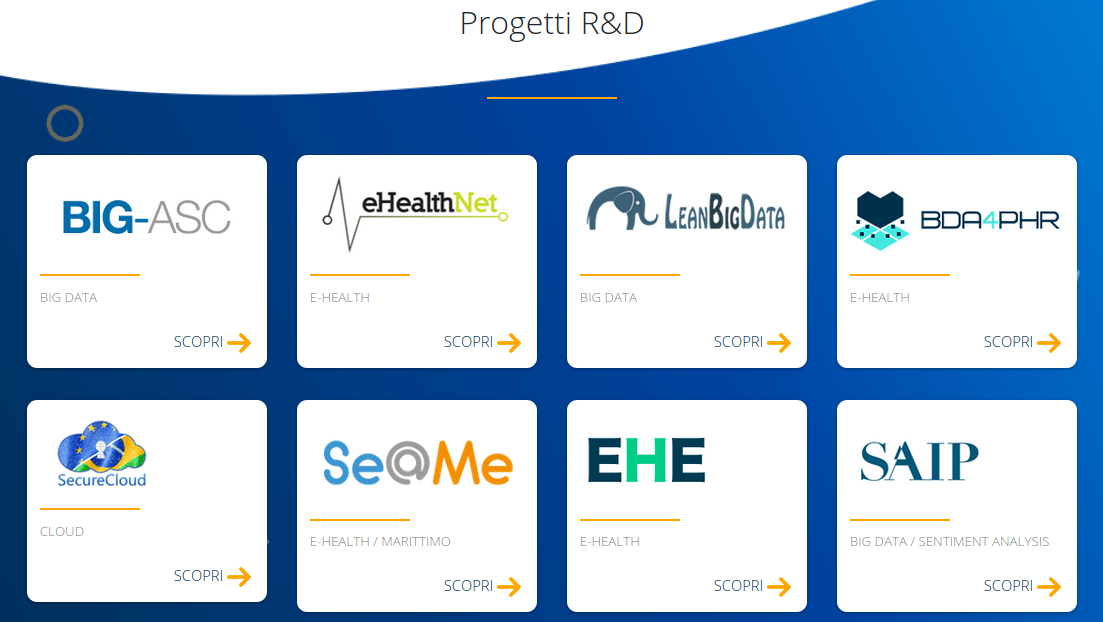
\includegraphics[height=5.5cm]{immagini/progetti}
  \captionof{figure}{I progetti di ricerca e sviluppo a cui Sync Lab collabora.}
  \caption*{\textbf{Fonte:} synclab.it}
\end{minipage} \\

Sempre nell'ambito dell'innovazione, posso dire che l'azienda ha un atteggiamento molto propositivo e aperto alle nuove tecnologie: non è raro, infatti, che i collaboratori propongano l'utilizzo di nuovi linguaggi, \textit{framework} e strumenti per completare i servizi e i prodotti offerti dall'azienda. \\
Ho potuto respirare questo clima di apertura anche nell'ambito del mio tirocinio: avendo avuto accesso alla piattaforma \textit{Discord} aziendale, ho potuto notare che il \textit{server} è diviso in più sottocanali, ognuno dedicato a un ambito di sviluppo, in cui i dipendenti inoltrano articoli e documentazione riguardanti nuove tecnologie, aprendo così a un dibattito costruttivo.
